\section*{Anhang}
\addcontentsline{toc}{section}{Anhang}
\subsection*{Anhang A - Umfrage im Unternehmen}
\addcontentsline{toc}{subsection}{Anhang A - Umfrage im Unternehmen}
\label{kap:anhang1}
In diesem Kapitel sind die Details der in Kapitel \ref{kap:Umfrage} durchgeführten Umfrage abgebildet. Dazu wurden folgende Fragen gestellt:\\

\begin{xltabular}{\textwidth}{|P{0.03\textwidth}|p{0.465\textwidth}|P{0.465\textwidth}|}
    \hline
    \multicolumn{3}{|c|}{\textbf{Fragen zur Person}}\\\hline
    Nr. & Frage & Antwortmöglichkeiten \\\hline\hline
    1 & Welche Position nimmst bei adesso orange ein? & Höher; Manager; Senior Consultant; Consultant; Junior Consultant; Trainee;\\\hline
    2 & Welche Rolle hast du bereits in einem S/4HANA Transformationsprojekt eingenommen? & Projektleiter; Teilprojektleiter; Berater; Entwickler; Sonstiges;\\\hline
    3 & Wie viele Jahre Berufserfahrung hast du im SAP-Bereich? & mehr als 10 Jahre; 7-10 Jahre; 4-6 Jahre; 1-3 Jahre; weniger als 1 Jahr;\\\hline
    4 & In wie vielen Projekten mit Anwendung der \glqq{}adesso active transformation\grqq{} hast du bereits mitgearbeitet? & mehr als 5 Projekten; 3-5 Projekten; 2-3 Projekten; 1 Projekt; Kein Projekt;\\\hline\hline
    \multicolumn{3}{|c|}{\textbf{Fragen zum Business Transformation Tracker}}\\\hline
    5 & Ich habe bereits häufig mit dem Business Transformation Tracker (bzw. der Tracebility Matrix) gearbeitet. & Ich stimme voll zu; Ich stimme eher zu; Neutral; Ich stimme eher nicht zu; Ich stimme nicht zu;\\\hline
    6 & Ich arbeite gerne mit dem Business Transformation Tracker. & Ich stimme voll zu; Ich stimme eher zu; Neutral; Ich stimme eher nicht zu; Ich stimme nicht zu;\\\hline
    7 & Der Funktionsumfang des Business Transformation Tracker ist ausreichend. & Ich stimme voll zu; Ich stimme eher zu; Neutral; Ich stimme eher nicht zu; Ich stimme nicht zu;\\\hline
    8 & Der Business Transformation Tracker belastet mehr, als er nutzt. & Ich stimme voll zu; Ich stimme eher zu; Neutral; Ich stimme eher nicht zu; Ich stimme nicht zu;\\\hline
    9 & Ich komme mit der aktuellen Umsetzung des Business Transformation Tracker gut zurecht. & Ich stimme voll zu; Ich stimme eher zu; Neutral; Ich stimme eher nicht zu; Ich stimme nicht zu;\\\hline
    10 & Ich sehe Verbesserungspotenziale im Business Transformation Tracker. & Ich stimme voll zu; Ich stimme eher zu; Neutral; Ich stimme eher nicht zu; Ich stimme nicht zu;\\\hline
    11 & Ich sehe den Business Transformation Tracker als gutes Mittel zum Ziel. & Ich stimme voll zu; Ich stimme eher zu; Neutral; Ich stimme eher nicht zu; Ich stimme nicht zu;\\\hline
    12 & Ich würde den Business Transformation Tracker anderen Kollegen weiterempfehlen. & Ich stimme voll zu; Ich stimme eher zu; Neutral; Ich stimme eher nicht zu; Ich stimme nicht zu;\\\hline\hline
    \multicolumn{3}{|c|}{\textbf{Verbesserungsvorschläge und Ideen}}\\\hline
    13 & Welche Verbesserungsvorschläge für die bestehende Version des Business Transformation Tracker hast du? & Freitextfeld\\\hline
    14 & Hast du Vorschläge um den Funktionsumfang des Business Transformation Tracker zu erweitern? & Freitextfeld\\\hline
    15 & Hast du sonstige Anmerkungen? & Freitextfeld\\\hline
    16 & Ich stehe für Rückfragen zur Verfügung. & Ja; Nein;\\\hline
    17 & Hier hast du die Möglichkeit deine Kontaktdaten zu hinterlassen. & Freitextfeld\\\hline
\end{xltabular}
\newpage
\subsection*{Anhang B - Ergebnisse der Umfrage}
\addcontentsline{toc}{subsection}{Anhang B - Ergebnisse der Umfrage}
Zur verbesserten Anschauung sind die Abbildungen ebenfalls im Verzeichnis ./Bilder/Anhang B-Ergebnisse.png dieser Arbeit abgelegt.
\begin{figure}[h!]
    \centering
    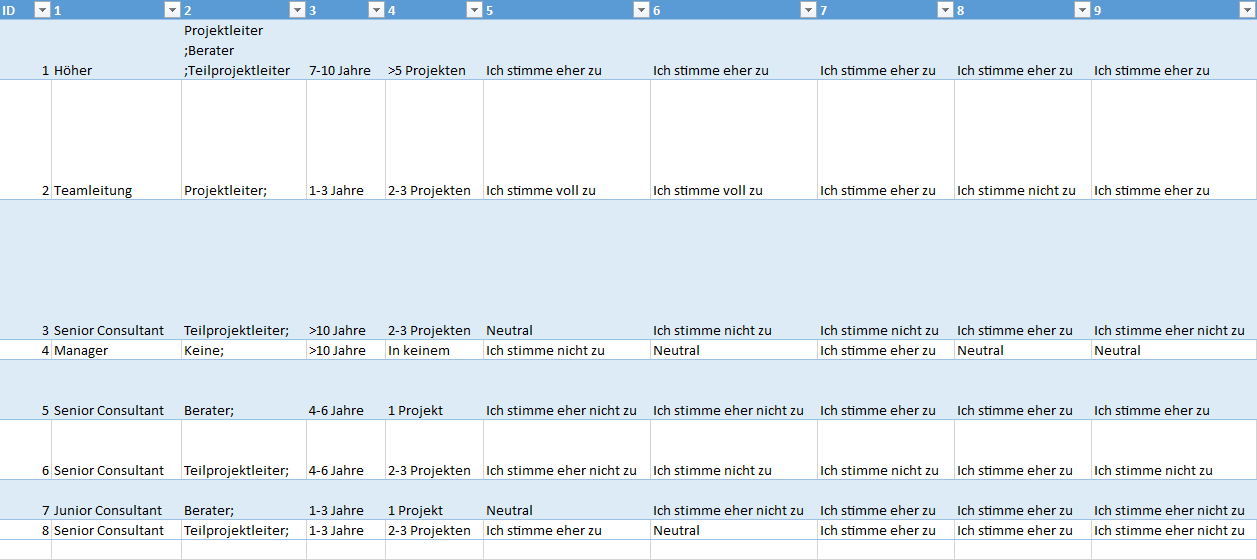
\includegraphics[angle=-90, scale=0.65]{./Bilder/Anhang B-Ergebnisse.png}
\end{figure}
\newpage
\begin{figure}[h!]
    \centering
    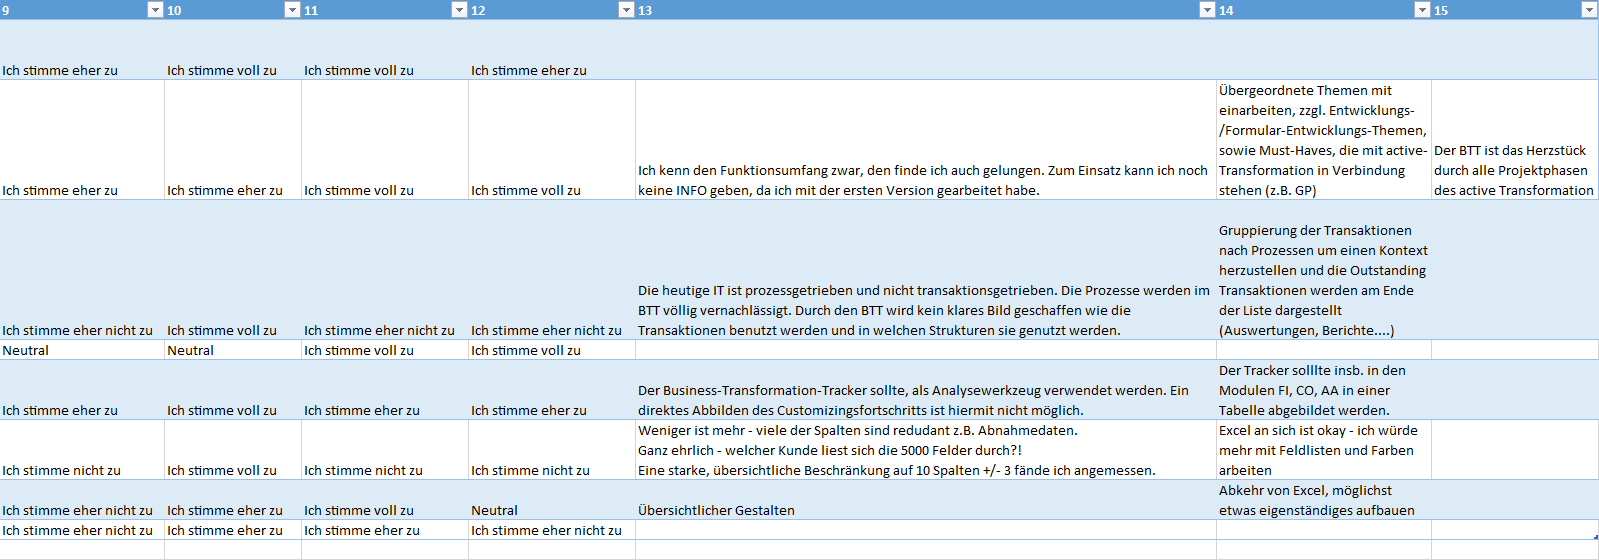
\includegraphics[angle=-90, scale=0.6]{./Bilder/Anhang B-Ergebnisse2.png}
\end{figure}
\newpage